\documentclass[12pt]{beamer}

\usetheme[progressbar=frametitle]{metropolis}

\usepackage{booktabs}
\usepackage[scale=2]{ccicons}
\usepackage[utf8]{inputenc}
\usepackage[german]{babel}
\usepackage{eurosym}
\usepackage{listings}
\usepackage{setspace}
\usepackage{pgfplots}
\usepgfplotslibrary{dateplot}

\usepackage{xspace}
\newcommand{\themename}{\textbf{\textsc{metropolis}}\xspace}

\newenvironment{changemargin}[2]{%
	\begin{list}{}{%
			\setlength{\topsep}{0pt}%
			\setlength{\leftmargin}{#1}%
			\setlength{\rightmargin}{#2}%
			\setlength{\listparindent}{\parindent}%
			\setlength{\itemindent}{\parindent}%
			\setlength{\parsep}{\parskip}%
		}%
		\item[]}{\end{list}}

\setbeamercolor{alerted text}{fg=red, bg=black}

\title{Fehlervorhersage in Java-Code mittels Machine Learning}
\date{\today}
\author{Tobias Meier (meierto3), Yacine Mekesser (mekesyac)}
\institute{ZHAW}
\titlegraphic{\hfill\includegraphics[height=1cm]{resources/images/de-zhaw-init-sw}}

\begin{document}

\maketitle

% * Was ist das für eine Präsentation (logisch)
% * Was ist unser Ziel/der Inhalt? -> Übersicht und Einführung in die Arbeit, keine technischen Details (dafür auf die Arbeit verweisen)

% http://www.landsiedel-seminare.de/rhetorik/rhetorik-standardaufbau-kurzvortrag-einleitung.html
% a) Anrede und Begrüßung des Publikums
% b) Vorstellung
% c) Nennung des Themas der Präsentation und Abgrenzung zu anderen Themen
% d) Inhalte und Ablauf kurz vorstellen
% e) Eigene fachliche Kompetenz darstellen
% f) Ziele der Präsentation nennen
% g) Praxisbezug herstellen

\begin{frame}{Inhaltsverzeichnis}
	\setbeamertemplate{section in toc}[sections numbered]
	\setstretch{2}
	\begin{columns}
		\begin{column}{0.5\textwidth}
			\tableofcontents[sections={1-6}]
		\end{column}
		\begin{column}{0.5\textwidth}
			\tableofcontents[sections={7-11}]
		\end{column}
	\end{columns}
\end{frame}


\section{Einleitung} % TOBI

\begin{frame}[fragile]{Softwarefehler I}
% Quelle: iX Studie 01/2006 Software-Testmanagement
\begin{itemize}
	\item \alert{\EUR{84.4 Mrd.}} jährliche Verluste in DE
\end{itemize}

\begin{figure}[h!]
	\centering
	\includegraphics[width=0.65\linewidth]{resources/images/ausgangslage_kostenzusammensetzung}
	\label{fig:ml_example}
\end{figure}

\end{frame}

\begin{frame}[fragile]{Softwarefehler II}
	Softwarefehler nehmen zu:
	\begin{itemize}
		\item Komplexität
		\item Wachsende Codebase
		\item Agile Softwareentwicklung
	\end{itemize}
	
\end{frame}

\begin{frame}[fragile]{Idee}
	\alert{Frühwarnsystem} für Softwarefehler
	
	\begin{itemize}
		\item Qualität
		\item Effizienz
		\item Günstiger
	\end{itemize}
\end{frame}

\begin{frame}[fragile]{Beobachtungen}
	\begin{itemize}
		\item Textverständnis mit Machine Learning
		\item Open-Source-Projekte
		\begin{itemize}
			\item Öffentliche Code Repositories
			\item Issue-Tracking-Systeme
		\end{itemize}
	\end{itemize}
\end{frame}

\begin{frame}[fragile]{Ansatz}
	\begin{itemize}
		\item Vorhersage von Bugs
		\item Codeanalyse mit ML
		\item Beschränkung auf Java-Projekte
	\end{itemize}
\end{frame}


% ca. 5min
\section{Grundlagen}	% YACINE

\begin{frame}[fragile]{Machine Learning}
	Ermöglicht Computern aus Beispielen zu \alert{lernen} und dann zu \alert{verallgemeinern}.
	\begin{figure}[h!]
		\centering
		\includegraphics[width=0.9\linewidth]{resources/images/ml_example}
		\label{fig:ml_example}
	\end{figure}
\end{frame}


\section{Vorgehen}	% TOBI

\begin{frame}[fragile]{Stand der Technik}
	Statischen Codeanalyse
	
	\begin{figure}[h!]
	\centering
	\includegraphics[width=1\linewidth]{resources/images/code_analysis_tools}
	\label{fig:staticcodeanalysis}
	\end{figure}

	
	Machine Learning
	\begin{itemize}
		\item Ideen und Potential vorhanden
		\item Keine schlüsselfertige Produkte
	\end{itemize}
	
\end{frame}

\begin{frame}[fragile]{Ziele}
	\begin{itemize}
		\item \alert{Grundstein} für weitere Arbeiten legen
		\item Toolset für \alert{projektbezogenes ML} bereitstellen
		\item Einbeziehung von \alert{Textanalyse-Features}
	\end{itemize}
\end{frame}

\begin{frame}[fragile]{Herausforderungen}
	\begin{itemize}
		\item ML Datensatz
		\begin{itemize}
			\item Code und Issue-Tracking
		\end{itemize}
		\item Features
		\item ML-Pipeline
	\end{itemize}
\end{frame}

% ca. 5 min
\section{Architektur}	% YACINE

\begin{frame}[fragile]{Lösungsansatz}
	Drei separate Tools:
	\begin{itemize}
		\item \alert{Repository Miner}
		\item \alert{Feature Extractor}
		\item \alert{ML-Pipeline}
	\end{itemize}
	
	Ermöglicht Modularität , Flexibilität \& Effizienz
\end{frame}

\begin{frame}[fragile]{Systemarchitektur}
	\begin{figure}[h!]
		\centering
		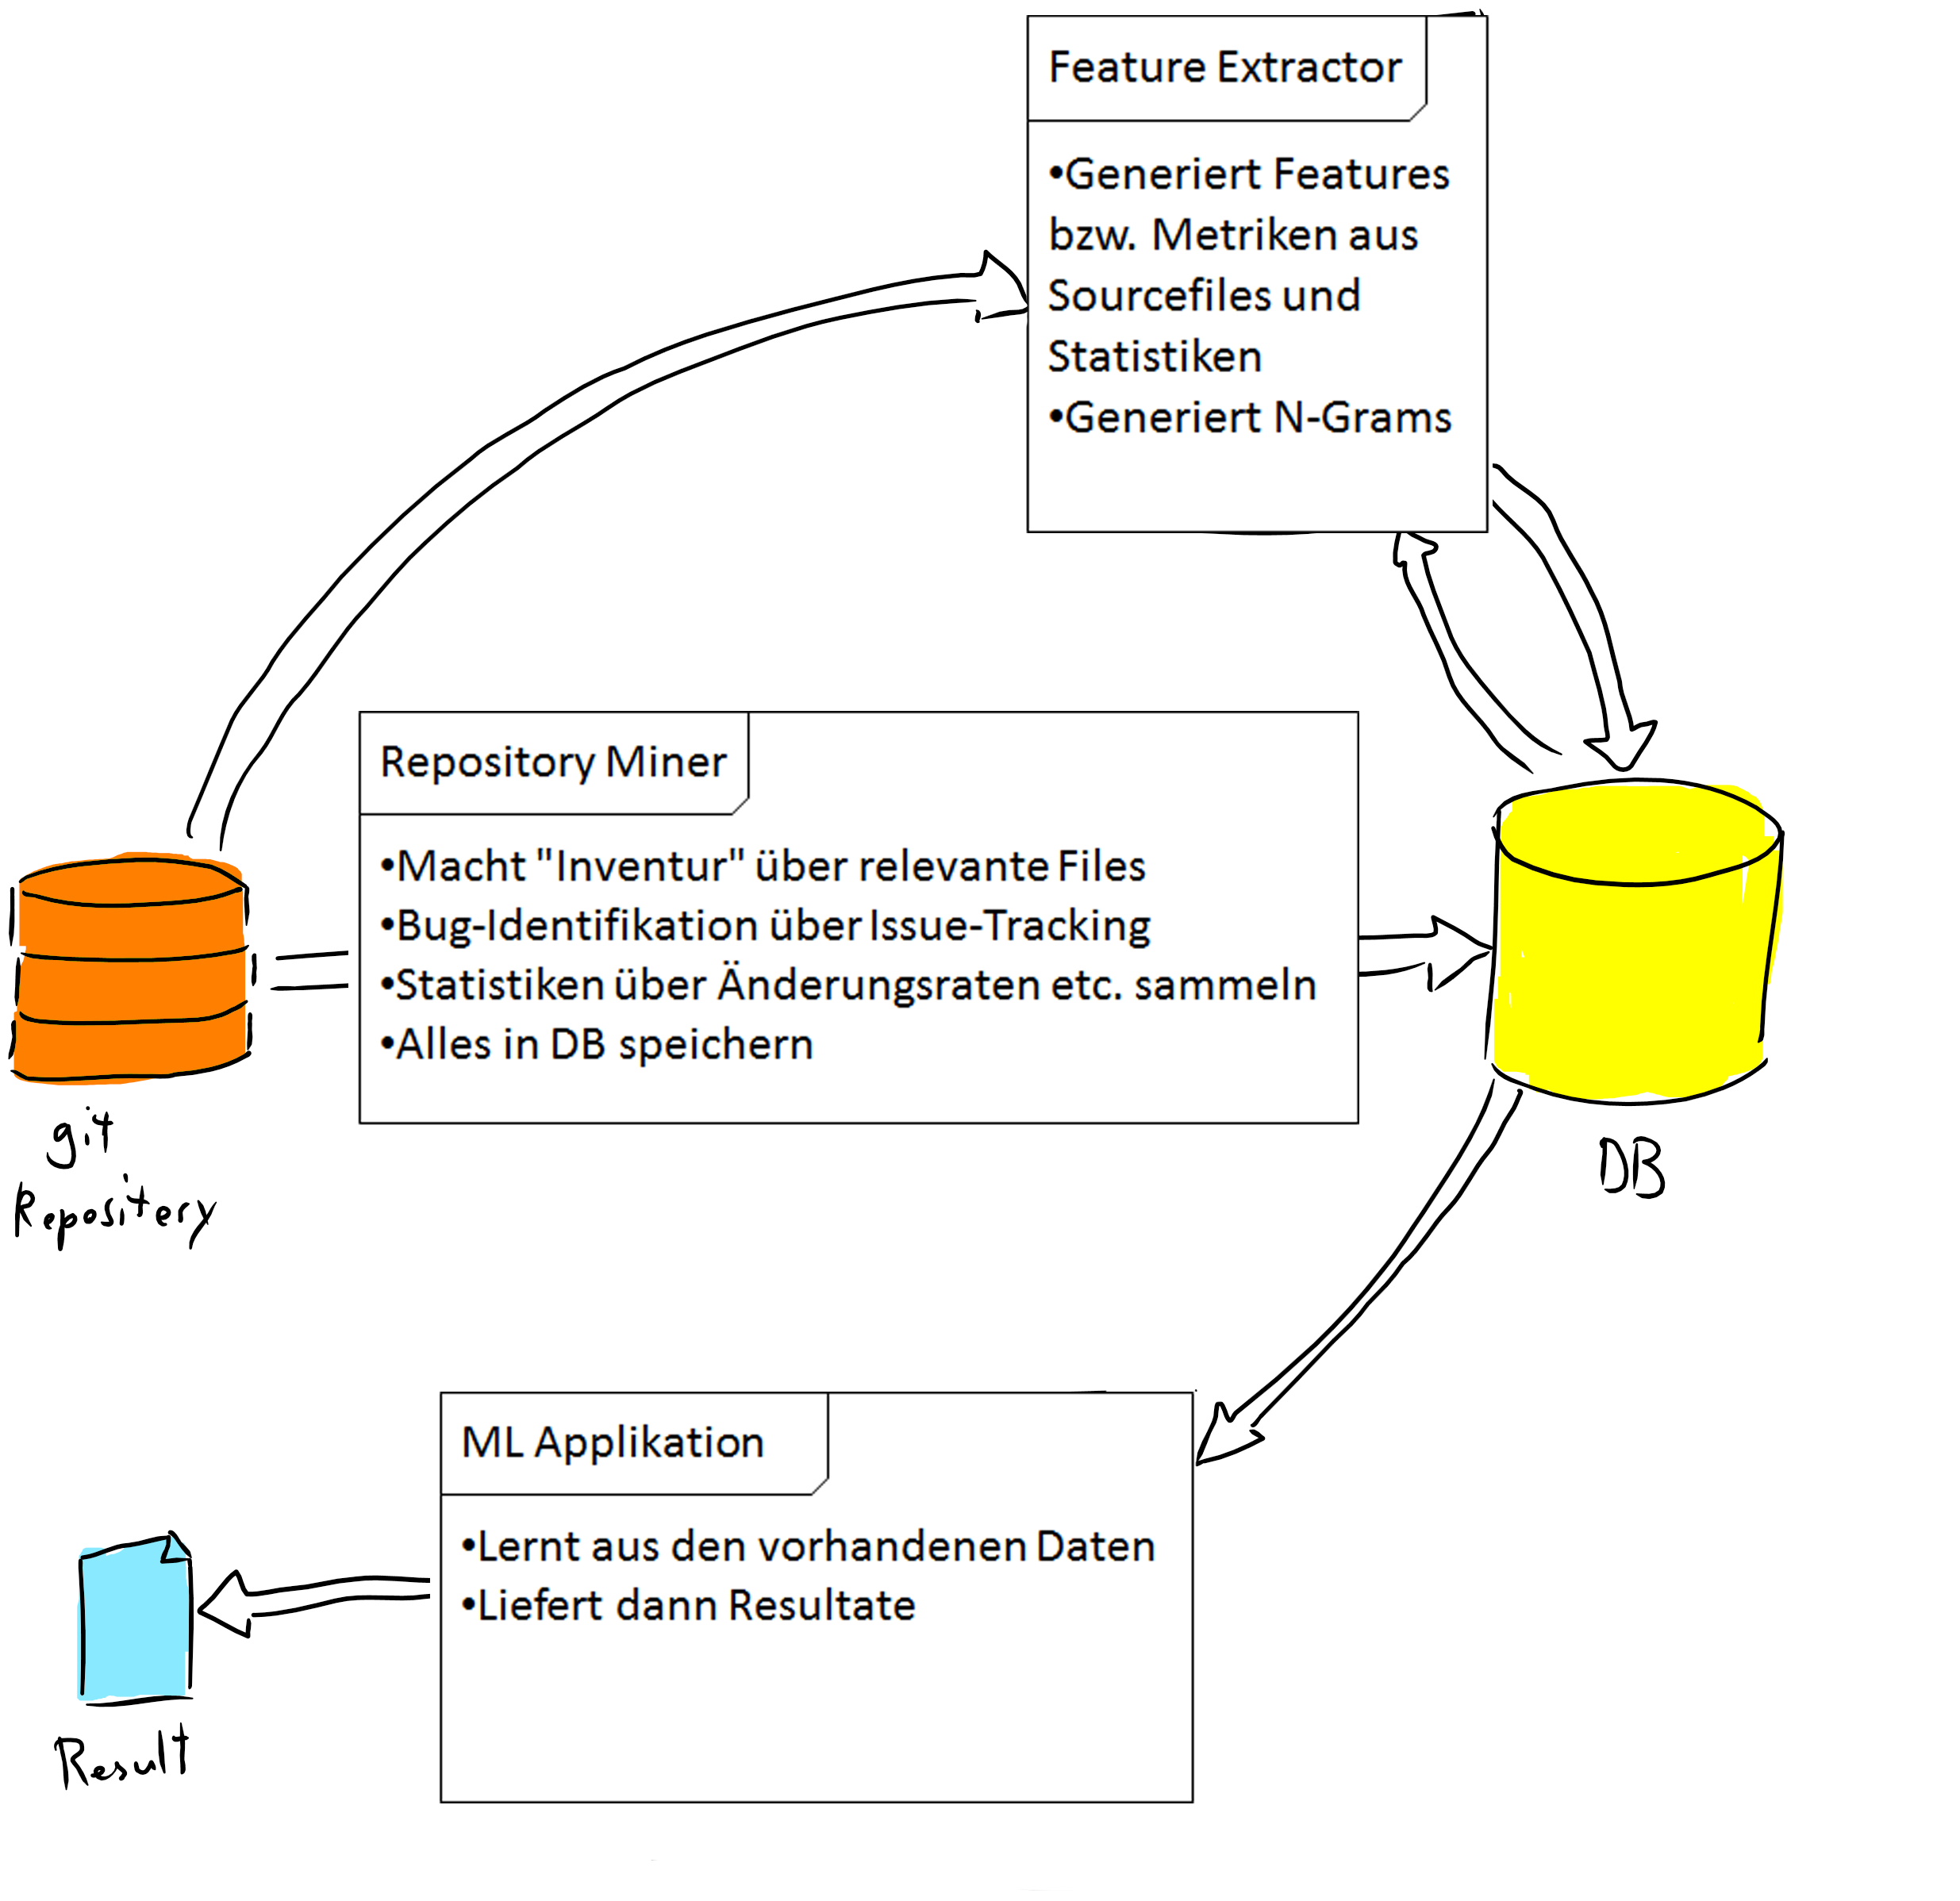
\includegraphics[width=1\linewidth]{resources/images/system_design}
		\label{fig:systemarchitektur}
	\end{figure}
\end{frame}


\section{Repository Miner}	% TOBI	

\begin{frame}[fragile]{Repository-Miner}
	\begin{itemize}
		\item Anbindung an Git, GitHub \& Jira
		\item Schnellen Zugriff bieten
		\item Daten strukturiert und normalisiert speichern
	\end{itemize}
	\begin{figure}[h!]
		\centering
		\includegraphics[width=1\linewidth]{resources/images/repo_miner_products}
	\end{figure}
\end{frame}


\begin{frame}[fragile]{Herausforderungen}
	\begin{figure}[h!]
		\centering
		\includegraphics[width=1\linewidth]{resources/images/Link-Issue-to-Bug}
		\label{fig:link-issue-to-bug}
	\end{figure}
\end{frame}


\begin{frame}[fragile]{Workflow}
	\begin{figure}[h!]
		\centering
		\includegraphics[width=1\linewidth]{resources/images/Repository-Miner-Ablauf}
	\end{figure}
\end{frame}

\begin{frame}[fragile]{Erkenntnisse I}
	\begin{changemargin}{-1cm}{-1cm}
		\begin{figure}[h!]
			\centering
			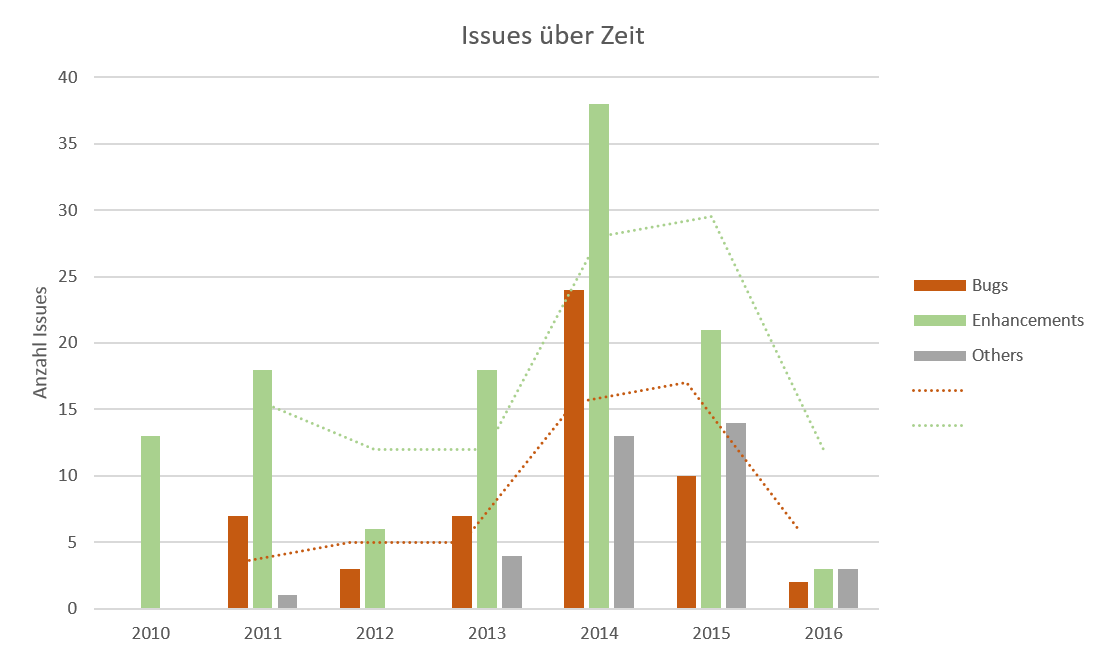
\includegraphics[width=1\linewidth]{resources/images/issues_over_time_internalengine}
		\end{figure}
	\end{changemargin}
\end{frame}

\begin{frame}[fragile]{Erkenntnisse II}
	\begin{changemargin}{-1cm}{-1cm}
		\begin{figure}[h!]
			\centering
			\includegraphics[width=1\linewidth]{resources/images/internal_engine_2014}
		\end{figure}
	\end{changemargin}
\end{frame}

\section{Features} % TOBI

%TODO Einstieg Features. Was ist das??? (Siehe Einleitung Machine Learning)

\begin{frame}[fragile]{Features}
	\begin{itemize}
		\item Messbare Eigenschaften einer Beobachtung
	\end{itemize}
	\begin{figure}[h!]
		\centering
		\includegraphics[width=1\linewidth]{resources/images/ml_example}
		\label{fig:ml_example}
	\end{figure}
\end{frame}

\begin{frame}[fragile]{Feature-Gruppen}
	\begin{itemize}
		\item Lines-of-Code-Features
		\item Objektorientierte Features
		\item Code-Complexity-Features
		\item Anzahl-und-Typen-Features
		\item Temporale Features
		\item Länge-von-Namen-Features
	\end{itemize}
\end{frame}

\begin{frame}[fragile]{N-Grams}
	\begin{itemize}
		\item Bug-Mustererkennung
		\item Verschiedene Abstraktionslevels
	\end{itemize}
	\begin{lstlisting}[frame=single,label={lst:ngrams}]
Code (Java): public class MyClass..
	
Code (AST): 
(55, TypeDeclaration)
  (83, Modifier)
    (43, SimpleType)
      (42, SimpleName)
	
N-Gram: 55_83_43_42
	\end{lstlisting}
\end{frame}

\begin{frame}[fragile]{Feature Extractor}
	\begin{itemize}
		\item Berechnet Features aus der Datenbasis
		\item AST-Parsing
		\item Modularer Aufbau
	\end{itemize}
\end{frame}


% ca. 6 min
\section{ML-Pipeline} % YACINE

\begin{frame}[fragile]{Herausforderungen}
	\begin{itemize}
		\item Umgang mit \alert{grossen Datensets}
		\begin{itemize}
			\item Datenset-Caching
			\item Sparse-Matrizen
		\end{itemize}
		\item Einfache Konfiguration verschiedener \alert{ML-Algorithmen}
		\begin{itemize}
			\item Zentrales Config-File
		\end{itemize}
		\item Resultate müssen \alert{bewertet} und \alert{analysiert} werden
		\begin{itemize}
			\item Verschiedene Charts \& Reports
		\end{itemize}
	\end{itemize}
\end{frame}


\begin{frame}[fragile]{Workflow}
	\begin{figure}[h!]
		\centering
		\includegraphics[width=1\linewidth]{resources/images/ml_pipeline_workflow}
		\label{fig:ml_comparisation_runtime}
	\end{figure}
\end{frame}


\section{Demo}	% TOBI & YACINE
\begin{frame}[fragile]{Testdaten}
	\begin{itemize}
		\item Projekt: \alert{Elasticsearch}
		\begin{itemize}
			\item $> 6$ Jahre
			\item $\sim 22\,000$ Commits
			\item $\sim 10\,000$ Issues (GitHub)
		\end{itemize}
		\item Trainingsset: 01.10.2014 - 31.12.2014
		\begin{itemize}
			\item 620 Commits
			\item $3\,414$ Dateiversionen
		\end{itemize}
		\item Testset: 01.01.2015 - 31.01.2015 
		\begin{itemize}
			\item 165 Commits
			\item 950 Dateiversionen
		\end{itemize}
	\end{itemize}
\end{frame}

\begin{frame}[fragile]{Workflow der ML-Pipeline}
	\begin{figure}[h!]
		\centering
		\includegraphics[width=1\linewidth]{resources/images/ml_pipeline_workflow}
		\label{fig:ml_comparisation_runtime}
	\end{figure}
\end{frame}


\section{Resultate}	% YACINE

\begin{frame}[fragile]{Vergleich von ML-Algorithmen}
	\begin{figure}[h!]
		\centering
		\includegraphics[width=1\linewidth]{resources/images/ml_vergleich_mde}
	\end{figure}
\end{frame}

\begin{frame}[fragile]{Laufzeit von ML-Algorithmen}
	\begin{figure}[h!]
		\centering
		\includegraphics[width=1\linewidth]{resources/images/ml_vergleich_runtime}
	\end{figure}
\end{frame}

\begin{frame}[fragile]{Performance von N-Grams}
	\begin{figure}[h!]
		\centering
		\includegraphics[width=1\linewidth]{resources/images/ml_vergleich_ngrams}
	\end{figure}
\end{frame}

\begin{frame}[fragile]{Vergleich von Projekten}
	\begin{figure}[h!]
		\centering
		\includegraphics[width=1\linewidth]{resources/images/ml_vergleich_projekte}
	\end{figure}
\end{frame}

\section{Zusammenfassung}	% TOBI

\begin{frame}[fragile]{Diskussion}
	\begin{itemize}
		\item Tool-Set für projektbezogenes Lernen
		\item Grundlage für weitere Arbeiten
		\item Textanalyse-Features
		\item einige Experimente
	\end{itemize}
\end{frame}

\begin{frame}[fragile]{Ausblick}
	\begin{itemize}
		\item Heatmap
		\item Fehlerlokalisierung
		\item Andere Programmiersprachen
		\item Cloud-Anwendung
	\end{itemize}
\end{frame}

\section{Fragen und Diskussion}

\end{document}
